% Full-width architecture overview with two independent routing bands.
\begingroup
\begin{tikzpicture}[
  x=1cm,
  y=1cm,
  font=\sffamily\footnotesize,
  >=Latex,
  flow/.style={->, line width=0.85pt, draw=black!72},
  feature/.style={->, line width=0.9pt, draw=blue!68!black},
  guidance/.style={->, line width=0.9pt, dashed, draw=orange!86!black},
  band/.style={draw=black!18, rounded corners=2pt, fill=black!1},
  stage/.style={draw=blue!62!black, rounded corners=2pt, fill=blue!6,
    minimum width=20mm, minimum height=13mm, align=center, inner sep=1.5pt},
  merge/.style={draw=black!42, rounded corners=1.5pt, fill=black!4,
    minimum width=5.5mm, minimum height=8mm, align=center, inner sep=1pt},
  projection/.style={draw=teal!65!black, rounded corners=1.5pt, fill=teal!6,
    minimum width=16mm, minimum height=9mm, align=center, inner sep=1.5pt},
  decoder/.style={draw=violet!62!black, rounded corners=1.5pt, fill=violet!6,
    minimum height=10mm, align=center, inner sep=2pt},
  head/.style={draw=orange!78!black, rounded corners=1.5pt, fill=orange!9,
    minimum height=10mm, align=center, inner sep=2pt},
  tap/.style={draw=blue!72!black, fill=blue!12, minimum size=2.8mm, inner sep=0pt},
  note/.style={font=\sffamily\footnotesize, text=black!70}
]

% Encoder band.
\node[band, minimum width=102mm, minimum height=25mm, anchor=south west]
  at (1.95,4.75) {};
\node[font=\sffamily\small\bfseries, anchor=west] at (2.15,6.98)
  {Four-stage encoder};

\node[draw=black!45, fill=white, inner sep=1.0pt] (input) at (0.50,5.60)
  {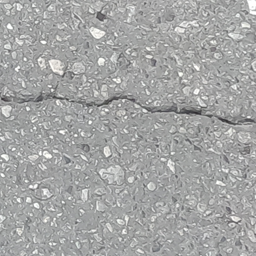
\includegraphics[width=8mm]{../dataset/CrackMap/test_img/GOPR0317 (5).png}};
\node[note, align=center, anchor=north] at ($(input.south)+(0,-0.10)$)
  {Input\\$512^2$};
\node[head, minimum width=9mm] (stem) at (1.55,5.60) {Stem\\$3{\to}16$};

\node[stage] (s1) at (3.05,5.60) {TransMixer\\\textbf{GAB}\\$16,\ 128^2$};
\node[merge] (m1) at (4.40,5.60) {PM\\$\downarrow2$};
\node[stage] (s2) at (5.70,5.60) {TransMixer\\\textbf{GAB}\\$32,\ 64^2$};
\node[merge] (m2) at (7.05,5.60) {PM\\$\downarrow2$};
\node[stage] (s3) at (8.35,5.60) {TransMixer\\\textbf{GAB}\\$64,\ 32^2$};
\node[merge] (m3) at (9.70,5.60) {PM\\$\downarrow2$};
\node[stage] (s4) at (11.00,5.60) {TransMixer\\\textbf{GAB}\\$128,\ 16^2$};

\draw[flow] (input) -- (stem);
\draw[flow] (stem) -- (s1);
\draw[flow] (s1) -- (m1);
\draw[flow] (m1) -- (s2);
\draw[flow] (s2) -- (m2);
\draw[flow] (m2) -- (s3);
\draw[flow] (s3) -- (m3);
\draw[flow] (m3) -- (s4);

% Dedicated vertical ports prevent encoder-to-decoder paths from sharing lines.
\node[tap] (f1) at (3.05,4.42) {};
\node[tap] (f2) at (5.70,4.42) {};
\node[tap] (f3) at (8.35,4.42) {};
\node[tap] (f4) at (11.00,4.42) {};
\node[note, anchor=east] at ($(f1.west)+(-0.05,0)$) {$F_1$};
\node[note, anchor=east] at ($(f2.west)+(-0.05,0)$) {$F_2$};
\node[note, anchor=east] at ($(f3.west)+(-0.05,0)$) {$F_3$};
\node[note, anchor=east] at ($(f4.west)+(-0.05,0)$) {$F_4$};
\draw[feature] (s1.south) -- (f1);
\draw[feature] (s2.south) -- (f2);
\draw[feature] (s3.south) -- (f3);
\draw[feature] (s4.south) -- (f4);

\node[projection] (p1) at (3.05,3.62) {$1{\times}1$ proj.\\$16{\to}8$};
\node[projection] (p2) at (5.70,3.62) {$1{\times}1$ proj.\\$32{\to}8$};
\node[projection] (p3) at (8.35,3.62) {$1{\times}1$ proj.\\$64{\to}8$};
\node[projection] (p4) at (11.00,3.62) {$1{\times}1$ proj.\\$128{\to}8$};
\draw[feature] (f1) -- (p1);
\draw[feature] (f2) -- (p2);
\draw[feature] (f3) -- (p3);
\draw[feature] (f4) -- (p4);

% Decoder band.
\node[band, draw=violet!22, fill=violet!1, minimum width=129mm,
  minimum height=32mm, anchor=south west] at (0.35,-0.25) {};
\node[font=\sffamily\small\bfseries, text=violet!68!black, anchor=east]
  at (13.05,2.70) {SRF decoder};

\node[decoder, minimum width=19mm] (up1) at (1.52,2.02)
  {$F_1$ upsample\\to $512^2$};
\node[decoder, minimum width=21mm] (att) at (3.88,2.02)
  {Spatial attention\\$A=\sigma(\phi(F_1))$};
\node[decoder, minimum width=32mm] (align) at (7.30,2.02)
  {Align $F_{2:4}$ to $128^2$\\calibrate by $A$, then upsample};
\node[decoder, minimum width=14mm] (cat) at (7.30,0.72) {Concat\\$32$ ch};
\node[decoder, minimum width=16mm] (fuse) at (9.15,0.72)
  {Conv + GN\\$32{\to}8$};
\node[head, minimum width=14mm] (pred) at (10.92,0.72)
  {Prediction\\head};
\node[draw=black!45, fill=white, inner sep=1.0pt] (output) at (12.32,0.72)
  {\includegraphics[width=7.5mm]{../results/probability_maps/triple_stack_v4_crackmap/validate_v3_msa_ocv_gbc_seed42/GOPR0317 (5)_pre.png}};
\node[note, align=center, anchor=north] at ($(output.south)+(0,-0.09)$)
  {Probability map};

\draw[feature] (p1.south) -- ++(0,-0.20) -| (up1.north);
\draw[guidance] (p1.south east) -- ++(0,-0.38) -| (att.north);
\draw[feature] (p2.south) -- ++(0,-0.48) -| ([xshift=2mm]align.north west);
\draw[feature] (p3.south) -- ++(0,-0.31) -| (align.north);
\draw[feature] (p4.south) -- ++(0,-0.14) -| ([xshift=-2mm]align.north east);
\draw[guidance] (att.east) -- (align.west);
\draw[feature] (up1.south) -- ++(0,-0.55) -| (cat.west);
\draw[feature] (align.south) -- (cat.north);
\draw[flow] (cat) -- (fuse);
\draw[flow] (fuse) -- (pred);
\draw[flow] (pred) -- (output);

% Legend outside the data paths.
\draw[feature] (0.10,-0.52) -- (0.65,-0.52);
\node[note, anchor=west] at (0.72,-0.52) {feature};
\draw[guidance] (2.05,-0.52) -- (2.60,-0.52);
\node[note, anchor=west] at (2.67,-0.52) {$F_1$ guidance};

\end{tikzpicture}
\endgroup
